\subsection{UC-13}
\label{subsec:UC-13}

\begin{figure}[H]
    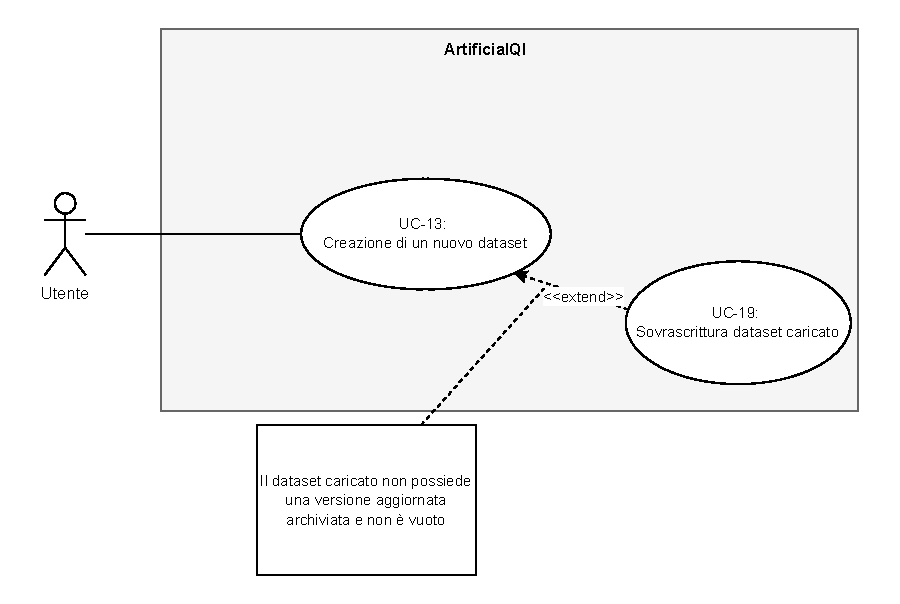
\includegraphics{Sezioni/UseCase/Immagini/UC-13.pdf}
    \caption{Diagramma UC-13.}
\end{figure}

\begin{usecase}{UC-13}{Creazione di un nuovo dataset temporaneo}

    \req{\hyperref[item:RU-3]{RU-3}} 

    \pre{
        \item Il sistema è attivo e funzionante
    }

    \post{
        \item Il nuovo dataset temporaneo viene caricato come dataset corrente
    }
    
    \actor{Utente}

    \subactors{}

    \trigger{L'utente deve creare un nuovo dataset}
    
    \inc{}

    \base{}

    \scenario{
        \item L'utente richiede la creazione di un nuovo dataset
        \item Viene creato un nuovo dataset temporaneo vuoto
        \item Il dataset temporaneo viene caricato come dataset corrente
    }

    \subscenario{
        \item[2.1] \textbf{Il dataset corrente non possiede una versione aggiornata archiviata e non è vuoto}
        \begin{itemize}
            \item[a.] \hyperref[subsec:UC-19]{UC-19}
        \end{itemize}
    }

\end{usecase}